\documentclass[tikz, border=20pt]{standalone}
\usepackage{amssymb,amsmath}
\usetikzlibrary{positioning, arrows.meta, fit, backgrounds, shapes.geometric}

\begin{document}
	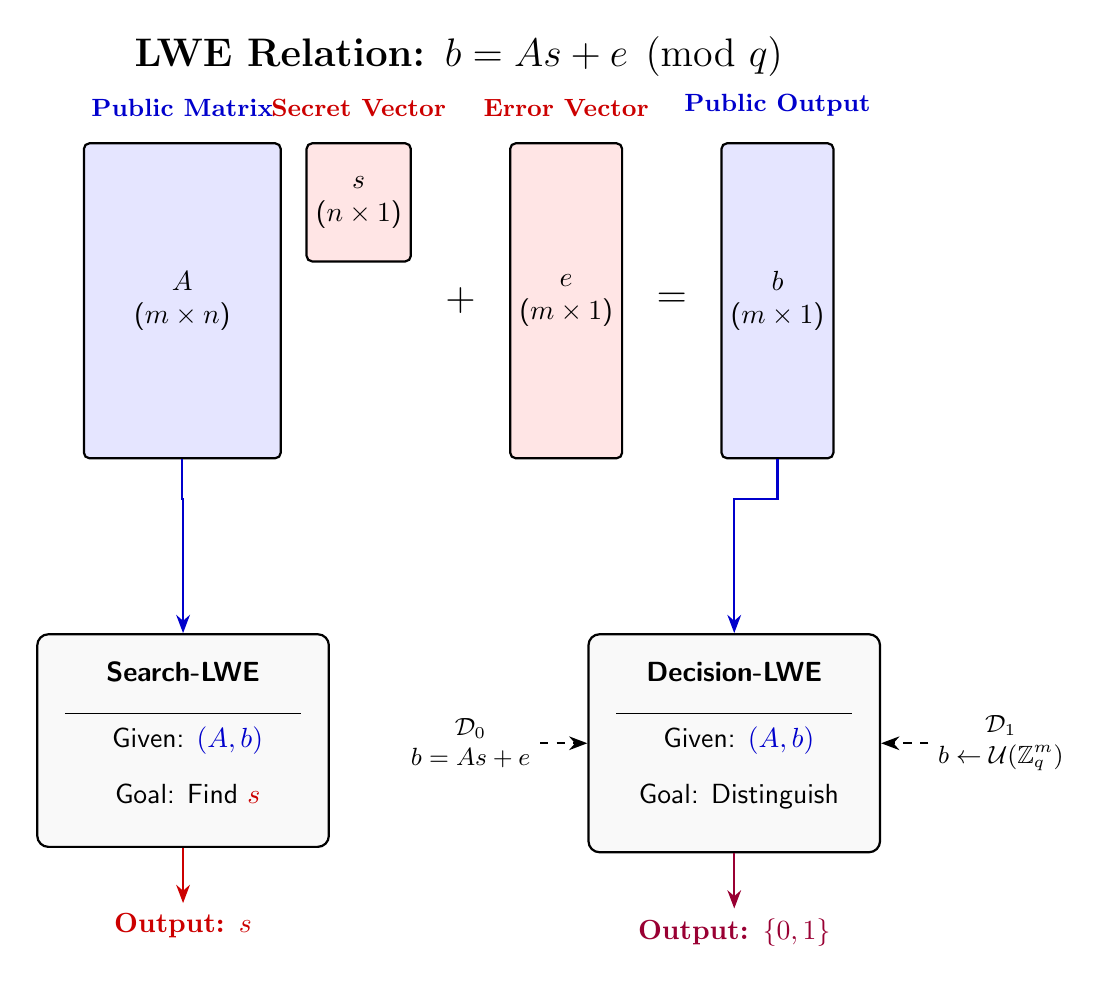
\begin{tikzpicture}[
		font=\sffamily,
		>=Stealth,
		public node/.style={draw, thick, fill=blue!10, rounded corners=2pt, align=center},
		secret node/.style={draw, thick, fill=red!10, rounded corners=2pt, align=center},
		op/.style={font=\Large\bfseries},
		box/.style={draw, thick, rounded corners, fill=gray!5, inner sep=10pt, align=center}
		]
		
		% ==========================================
		% 1. CORE LWE MATRIX EQUATION
		% ==========================================
		
		% Matrices and Vectors
		\node[public node, minimum width=2.5cm, minimum height=4cm] (A) {$A$\\($m \times n$)};
		\node[secret node, minimum width=0.8cm, minimum height=1.5cm, right=0.3cm of A, yshift=1.25cm] (s) {$s$\\($n \times 1$)};
		\node[op, right=0.3cm of s, yshift=-1.25cm] (plus) {$+$};
		\node[secret node, minimum width=0.8cm, minimum height=4cm, right=0.3cm of plus] (e) {$e$\\($m \times 1$)};
		\node[op, right=0.3cm of e] (eq) {$=$};
		\node[public node, minimum width=0.8cm, minimum height=4cm, right=0.3cm of eq] (b) {$b$\\($m \times 1$)};
		
		% Labels for Core LWE
		\node[above=0.2cm of A, text=blue!80!black, font=\small\bfseries] {Public Matrix};
		\node[above=0.2cm of s, text=red!80!black, font=\small\bfseries] {Secret Vector};
		\node[above=0.2cm of e, text=red!80!black, font=\small\bfseries] {Error Vector};
		\node[above=0.2cm of b, text=blue!80!black, font=\small\bfseries] {Public Output};
		
		% Grouping the equation
		\node[fit=(A) (s) (plus) (e) (eq) (b), inner sep=0.7cm] (lwe_eq) {};
		\node[above=0cm of lwe_eq, font=\Large\bfseries] {LWE Relation: $b = As + e \pmod q$};
		
		% ==========================================
		% 2. SEARCH LWE PROBLEM
		% ==========================================
		
		\node[box, below=1.5cm of lwe_eq, xshift=-3.5cm] (search) {
			\textbf{Search-LWE}\\
			\rule{3cm}{0.4pt}\\
			\vspace{0.2cm}
			Given: \textcolor{blue!80!black}{$(A, b)$}\\
			\vspace{0.2cm}
			Goal: Find \textcolor{red!80!black}{$s$}
		};
		
		% Arrow connecting public params to Search
		\draw[->, thick, blue!80!black] (A.south) -- ++(0,-0.5) -| (search.north);
		\draw[->, thick, red!80!black] (search.south) -- ++(0,-0.7) node[below, font=\bfseries] {Output: $s$};
		
		% ==========================================
		% 3. DECISION LWE PROBLEM
		% ==========================================
		
		\node[box, below=1.5cm of lwe_eq, xshift=3.5cm] (decision) {
			\textbf{Decision-LWE}\\
			\rule{3cm}{0.4pt}\\
			\vspace{0.2cm}
			Given: \textcolor{blue!80!black}{$(A, b)$}\\
			\vspace{0.2cm}
			Goal: Distinguish
		};
		
		% Distributions for Decision
		\node[left=0.6cm of decision, align=center, font=\small] (D0) {$\mathcal{D}_0$\\$b = As + e$};
		\node[right=0.6cm of decision, align=center, font=\small] (D1) {$\mathcal{D}_1$\\$b \leftarrow \mathcal{U}(\mathbb{Z}_q^m)$};
		
		% Arrows for Decision logic
		\draw[->, thick, dashed] (D0) -- (decision);
		\draw[->, thick, dashed] (D1) -- (decision);
		\draw[->, thick, blue!80!black] (b.south) -- ++(0,-0.5) -| (decision.north);
		\draw[->, thick, purple!80!black] (decision.south) -- ++(0,-0.7) node[below, font=\bfseries] {Output: $\{0, 1\}$};
		
	\end{tikzpicture}
\end{document}